\documentclass{article}
\usepackage{xeCJK}
\usepackage{graphicx}
\usepackage{color}
\usepackage[
	left=3.17cm,
	right=3.17cm,
	top=1.5cm,
	bottom=1.5cm
	]{geometry}
\definecolor{ustcblue}{cmyk}{1,0.8,0,0}
\title{USTC VI简要使用说明}
\author{ywg@USTC}
\date{}
\begin{document}
\maketitle
\section{版权问题及免责声明}
本素材库中所有图案、标识、文字及其组合的版权均归中国科学技术大学(或实际所有人)所有。

制作本素材库的目的仅仅是对一些合法的使用提供便利,素材库的作者及存储和下载服务提供者对使用本素材库所产生的后果不承担任何直接或间接责任。任何在本素材库的基础上进行的衍生、创作或其他任何行为所可能直接或间接引发的法律纠纷均由行为人承担相应法律责任,包括但不限于滥用学校标志、未经授权的商业使用以及恶意篡改等。

\section{简介}
USTC VI是一个用于\LaTeX{}内容创作或其他合法目的的中国科学技术大学视觉形象识别系统的免费矢量素材库。包含CorelDraw、eps和pdf版本的矢量素材,内容涵盖校徽、中英文校名及其组合等。

依照《中国科学技术大学视觉形象识别系统管理手册(试行)》的要求,本素材库对素材各个元素进行了精心调整设置,完全符合学校要求。其中针对\LaTeX{}系统进行了特殊优化,提供了简便的配色调整功能。

\section{\LaTeX{}用户使用方法简介}
\LaTeX{}用户可以直接使用原始配色的eps图片,也可以使用经过特殊修改的pdf版本的矢量图形自定义素材的颜色。

欲修改颜色,请将对应的pdf文件作为图片使用,并在使用时通过 \\
\verb|\textcolor{<color>}{\includegraphics[<some options>]{<ustc_logo_fig.pdf>}}| \\
来修改颜色。

所有的pdf图片都可以修改颜色,只需要换成对应的名字即可。

比如下面这些校名。

\noindent
\textcolor{ustcblue}{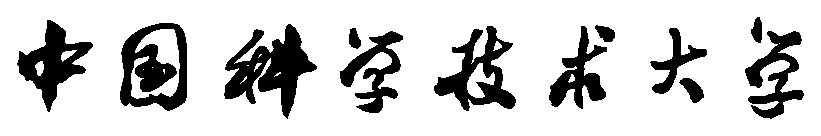
\includegraphics[width=\textwidth]{./pdffigures/ustc_logo_text.pdf}}
\textcolor{red}{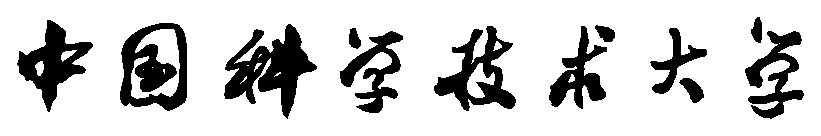
\includegraphics[width=\textwidth]{./pdffigures/ustc_logo_text.pdf}}
\textcolor{black}{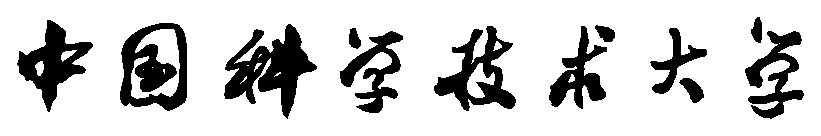
\includegraphics[width=\textwidth]{./pdffigures/ustc_logo_text.pdf}}

\section{下载}
下载地址: https://github.com/ustctug/ustclogo
下载方法参考通用论文模板下载方法。
\end{document}
